\documentclass[11pt, oneside]{article}   	% use "amsart" instead of "article" for AMSLaTeX format
\usepackage{geometry}                		% See geometry.pdf to learn the layout options. There are lots.
\geometry{letterpaper}                   		% ... or a4paper or a5paper or ... 
%\geometry{landscape}                		% Activate for rotated page geometry
%\usepackage[parfill]{parskip}    		% Activate to begin paragraphs with an empty line rather than an indent
\usepackage{graphicx}				% Use pdf, png, jpg, or eps§ with pdflatex; use eps in DVI mode
								% TeX will automatically convert eps --> pdf in pdflatex		
\usepackage{amssymb}

%SetFonts

%SetFonts


\title{Wiener Deconvolution}
\author{M. Gold}
\date{\today}							% Activate to display a given date or no date

\begin{document}
\maketitle
%\section{}
%\subsection{}
\begin{figure}[htbp] %  figure placement: here, top, bottom, or page
   \centering
   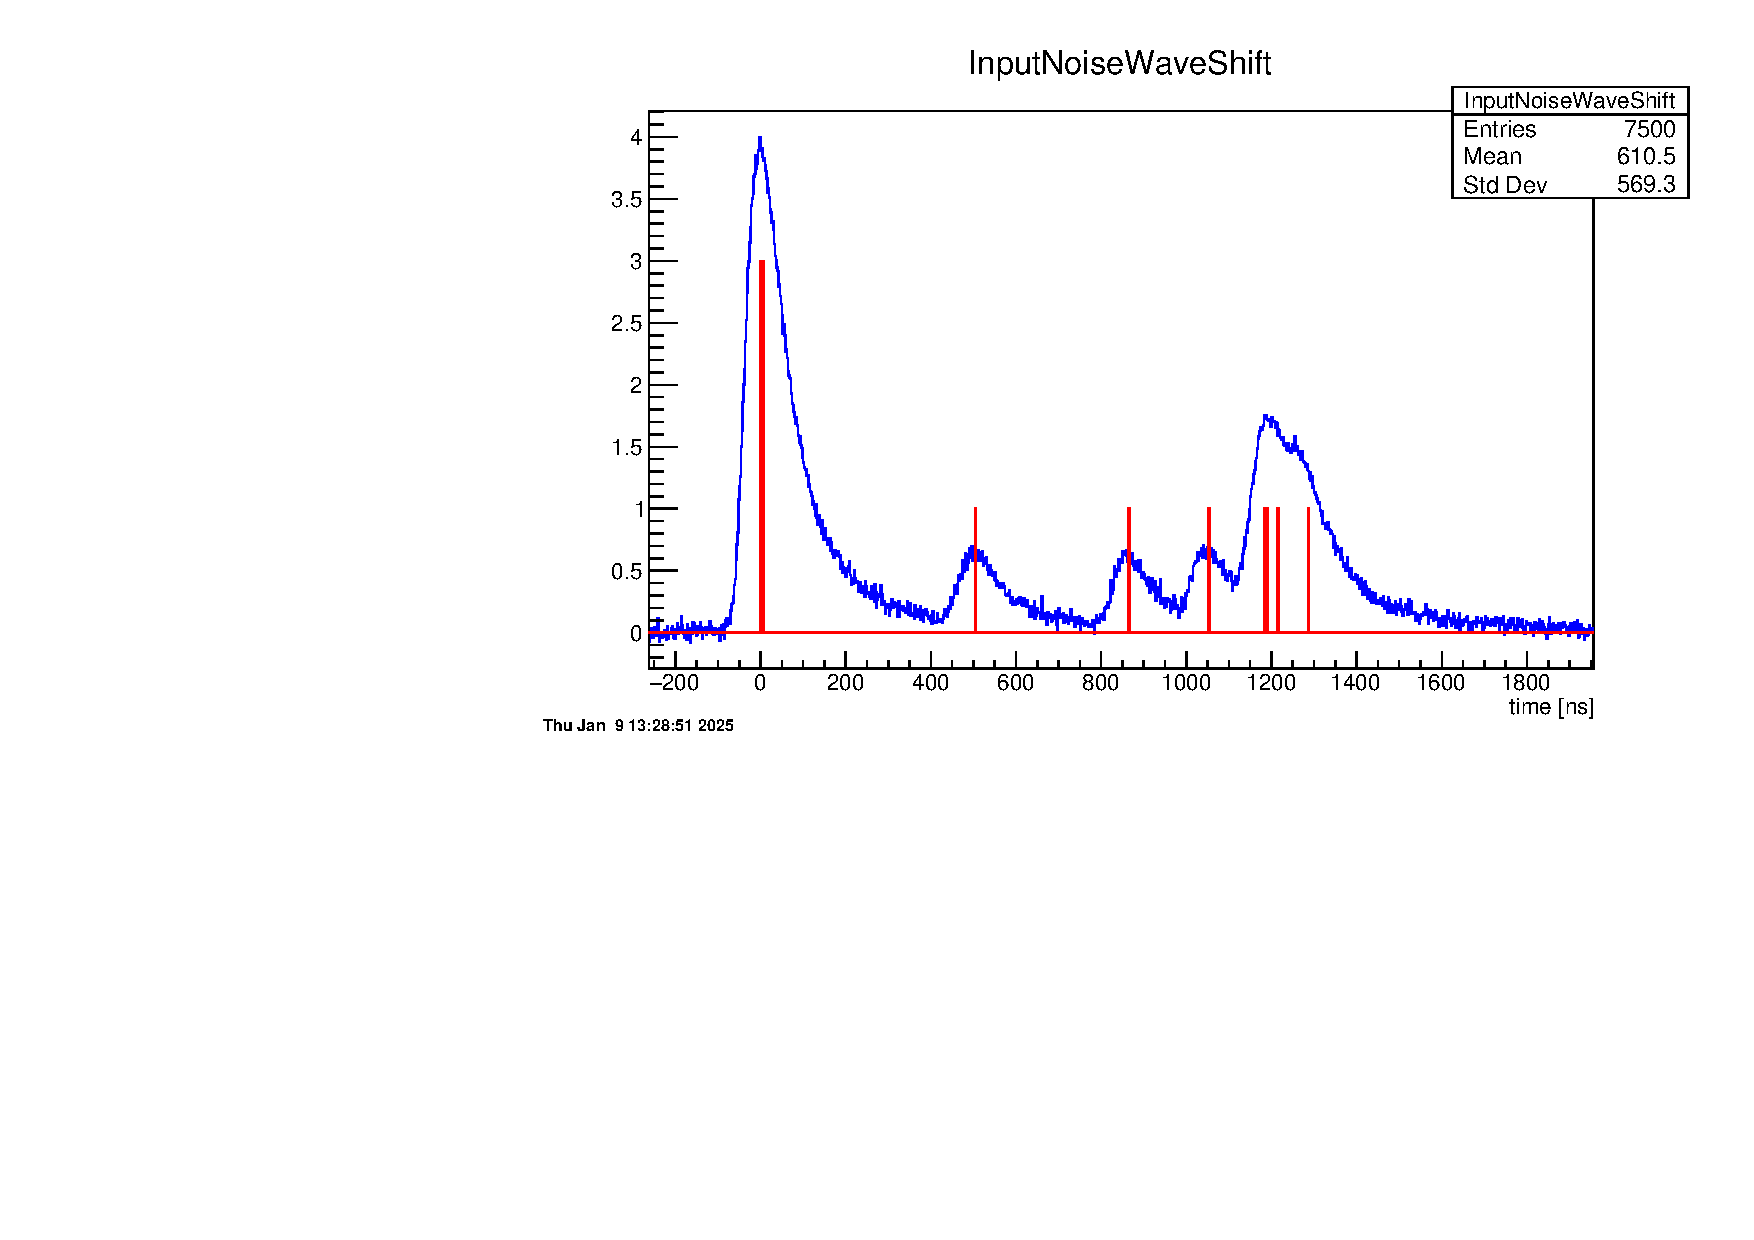
\includegraphics[width=0.9\linewidth]{input-4.00E-02-sigma-7500.pdf} 
   \caption{Similated data convoluted with Landau SIPM resolution}
   \label{fig:input}
\end{figure}


%\section{}
%\subsection{}
\begin{figure}[htbp] %  figure placement: here, top, bottom, or page
   \centering
   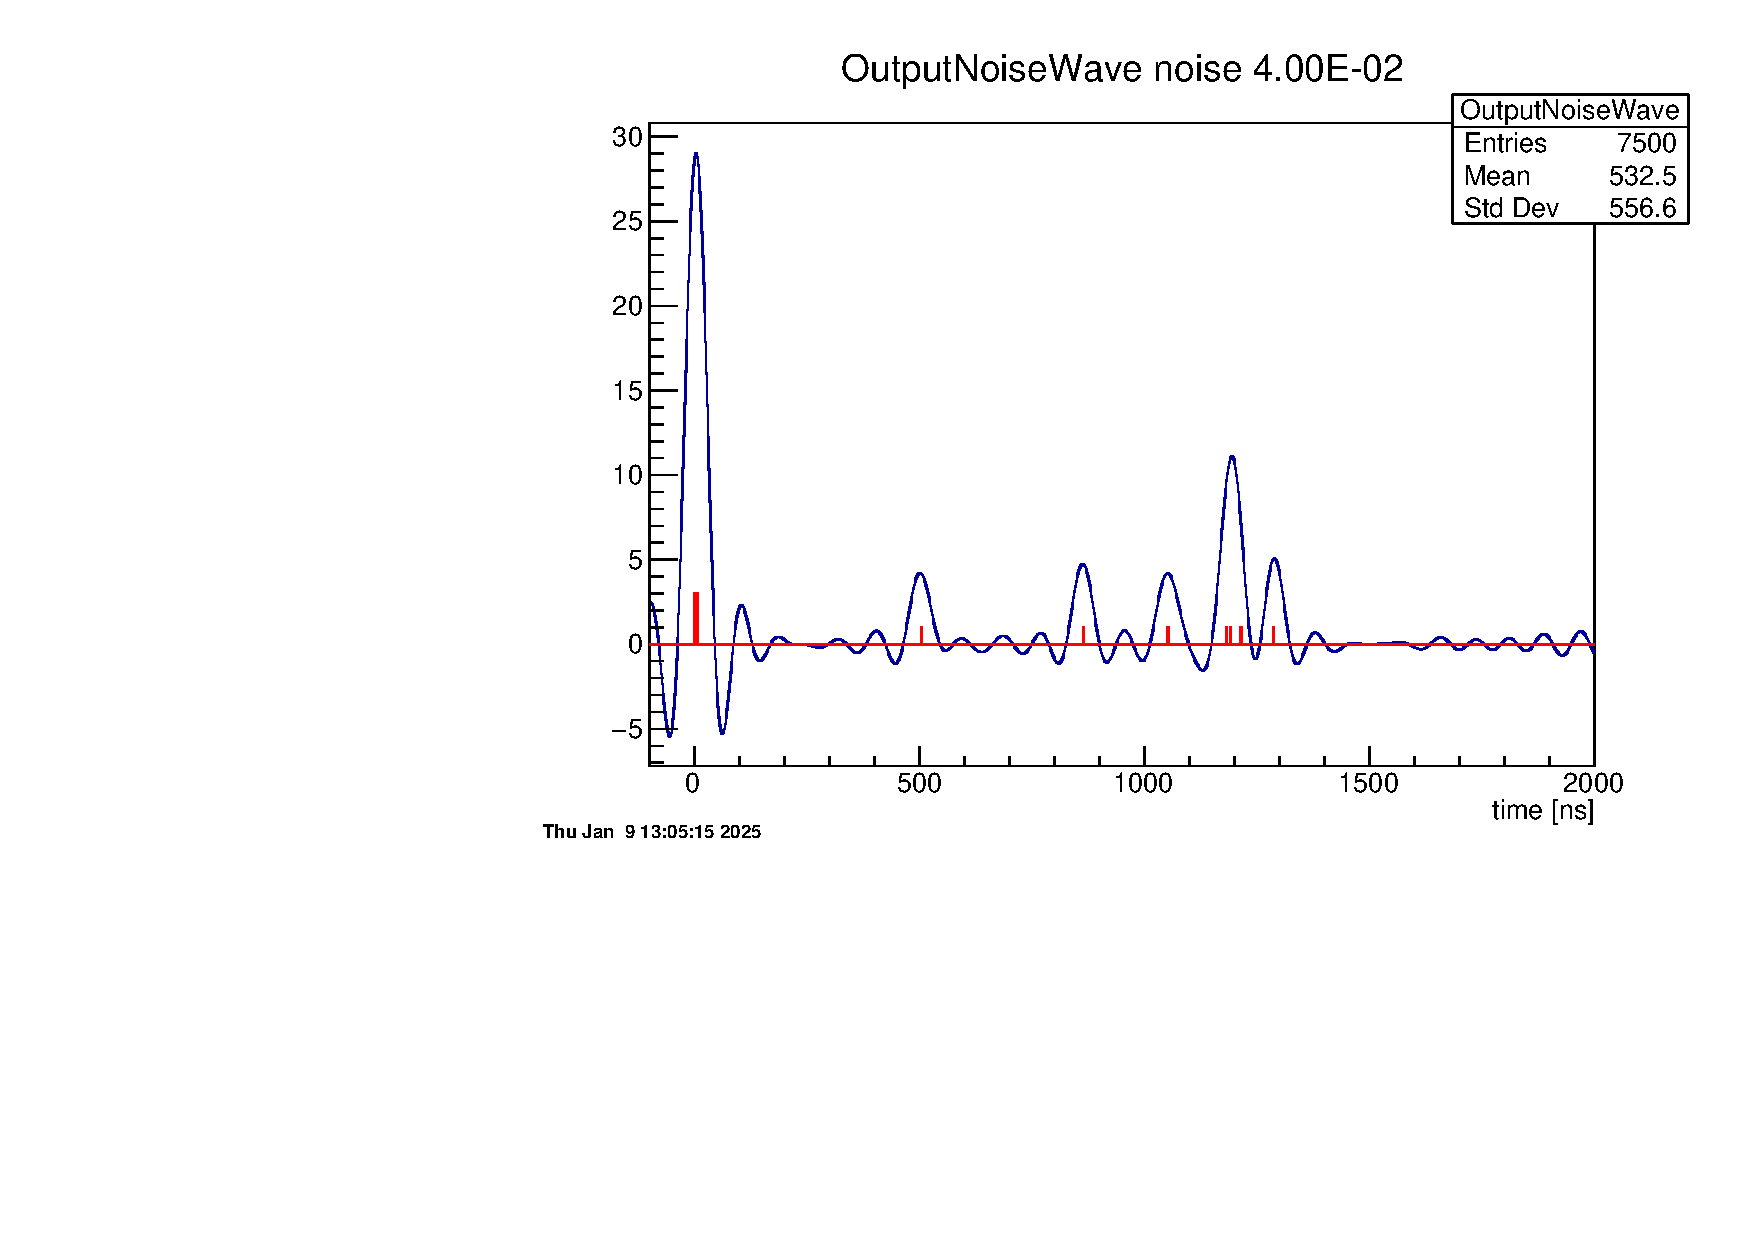
\includegraphics[width=0.9\linewidth]{outputNoise-4.00E-02-sigma-7500.pdf} 
   \caption{Wiener deconvoluted output with input photon distribution}
   \label{fig:input}
\end{figure}




\end{document}  
